\documentclass[a4paper,10pt]{paper}
\usepackage[utf8]{inputenc}
\usepackage{graphicx}
\usepackage{amsmath}

\setlength\textwidth{6.5in}
\setlength\oddsidemargin{0in}
\setlength\evensidemargin{0in}
% Title Page
\title{Architecture of E-Health Flanders platform}
\author{}

%TODO: stijl kiezen: componenten vet, interfaces /...
%TODO: Overal keys toevoegen.

\begin{document}
\maketitle

\part{Documentation Beyound Views}

\section{Documentation roadmap}

\subsection{Description of the parts}

\subsection{How stakeholders might use the package}

\subsubsection{Platform tester}

\subsubsection{Patient}

\subsubsection{Government}

\section{View template}

\section{System overview}

\section{Mapping between views}

\section{Directory}

\section{Glossary and acronym list}

\section{Background, design constraints, and rationale}



\part{Software Architecture Views}

\section{Module Uses View}

\subsection{Primary presentation}



\subsection{Element catalog}

\subsubsection{Elements and their properties}

\subsubsection{Relations and their properties}

\subsubsection{Element interfaces}

\subsubsection{Element behavior}

\subsection{Context diagram}

\subsection{Variability guide}

\subsection{Architecture background}

\subsubsection{Rationale}

\subsubsection{Analysis results}

\subsubsection{Assumptions}

\subsection{Other information}

\subsection{Related view packets}




\section{C\&C Client and Server View: Overview}

\subsection{Primary presentation}

\begin{center}
    \begin{figure}
      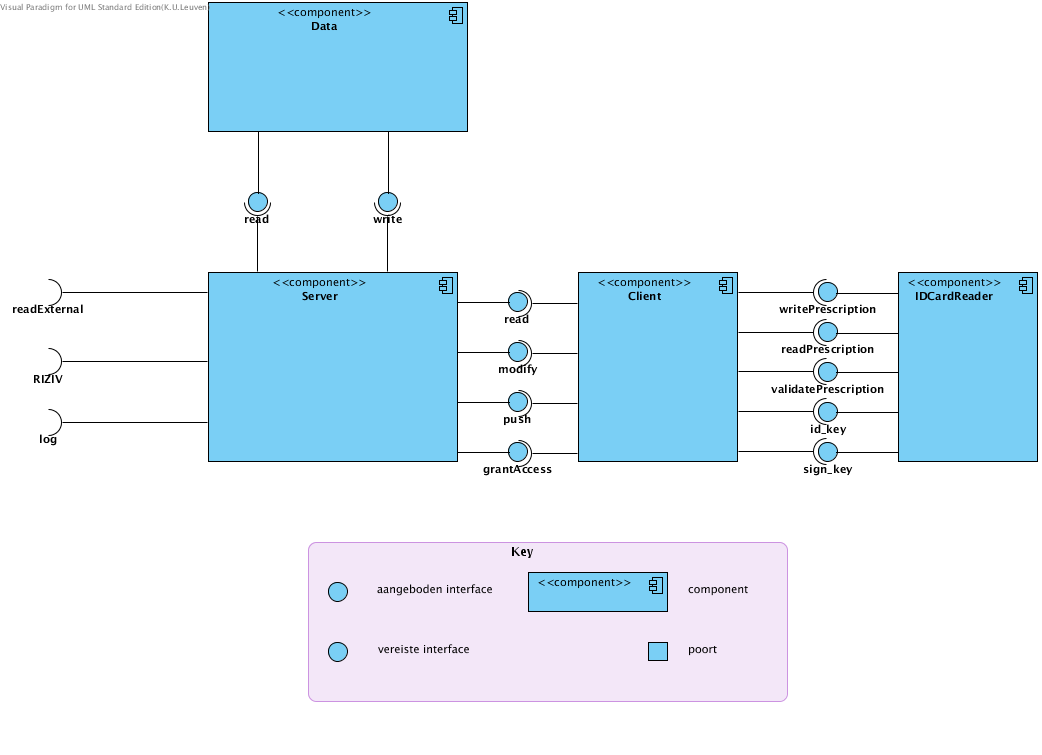
\includegraphics[width=\textwidth]{../images/ClientServer_Overview.png}
    \end{figure}
  \end{center}
%TODO opmaken figuur!


\subsection{Element catalog}

\paragraph{Server}
De server is de component waar clients verbinding mee maken.  De interacties tussen clients en servers gebeuren op een veilige manier.  De server is verbonden met clients, de overheid, eventuele externe componenten en de data server.  Meer informatie kan gevonden worden in \ref{Client and Server View: Server} Client and Server View: Server.
%TODO location

\paragraph{Client}
De client component is de component die gebruikers (dokters, pati\"{e}nten of apothekers) gebruiken om op een veilige manier met de server te interageren.  Meer informatie kan gevonden worden in \ref{Client and Server View: Client} Client and Server View: Client.
%TODO location

\paragraph{Data}
De data component is een database waar alle informatie zoals patienten dossiers en dokter data op bewaard zijn.  Hoe de data precies wordt opgeslaan is terug te vinden in het Deployment diagram.
%TODO location

\paragraph{Card}
De card component stelt de e-Card van de gebruiker voor.  De e-Card bevat gebruikersinformatie alsook twee keys.  Een key voor identificatie van de gebruiker en een key voor authenticatie.  Naast de gebruikersinformatie en de keys heeft de e-Card ook ruimte voor een aantal voorschriften op te slaan.  Meer informatie is terug te vinden in:
%TODO location

\paragraph{Government}
De government component bevat toegang tot de logging en RIZIV database.

\paragraph{External}
De external component bevat de validated data sources die gebruikers van de client kunnen opvragen via de server.

%TODO government en external => context diagram?


\subsection{Context diagram}
TODO
%TODO

\subsection{Variability guide}
[None]

\subsection{Architecture background}
%TODO

\subsubsection{Rationale}
Enkele design beslissingen die hier te zien zijn is het gebruik van de card reader voor het identifici\"{e}ren van de gebruikers op de centrale database, meer hierover is te vinden in het ...TODO.
%TODO security
%TODO voorschriften.

\subsection{Related view packets}
De volgende client-server views bekijken dit overview diagram in meer detail.  Ook in het deployment diagram is extra informatie te vinden vooral dan in verband met de opslag van de global medical records en dokter data.



\section{C\&C Client and Server View: Server}
\label{Client and Server View: Server}

\subsection{Primary presentation}

\begin{center}
    \begin{figure}
      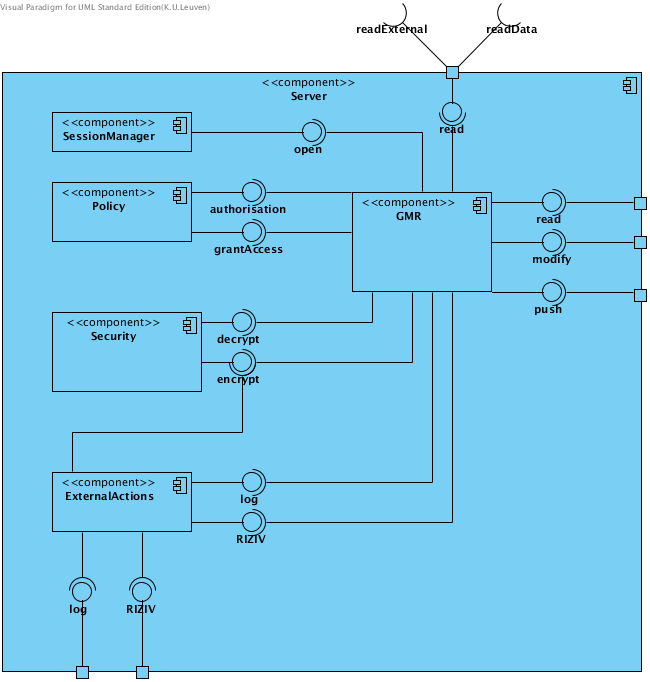
\includegraphics[width=\textwidth]{../images/ClientServer_Server.png}
    \end{figure}
  \end{center}
%TODO opmaken figuur!

\subsection{Element catalog}

\paragraph{GMR}
De GMR is de centrale component in de server component.  De GMR delegeert alle inkomende \textit{read}, \textit{modify} of \textit{push} acties naar de correcte andere componenten en doet dit uiteraard in de correcte volgorde.
%TODO: interactie diagram??

\subsubsection{Element interfaces} 

\paragraph{read}
TODO

\paragraph{modify}
TODO

\paragraph{push}
TODO

\subsubsection{Element behavior}
TODO

\paragraph{SessionManager}

\subsubsection{Element interfaces} 

\paragraph{open}
TODO

\subsubsection{Element behavior}
TODO

\paragraph{Policy}

\subsubsection{Element interfaces} 

\paragraph{autorisation}
TODO

\paragraph{grantAccess}
TODO

\subsubsection{Element behavior}
TODO

\paragraph{Security}

\paragraph{ExternalActions}

\subsubsection{Element interfaces} 

\paragraph{log}
TODO

\paragraph{RIZIV}
TODO

\subsection{Context diagram}

\subsection{Variability guide}

\subsection{Architecture background}

\subsubsection{Rationale}

\subsubsection{Analysis results}

\subsubsection{Assumptions}

\subsection{Other information}

\subsection{Related view packets}



\section{C\&C Client and Server View: Client}
\label{Client and Server View: Client}

\subsection{Primary presentation}

\begin{center}
    \begin{figure}
      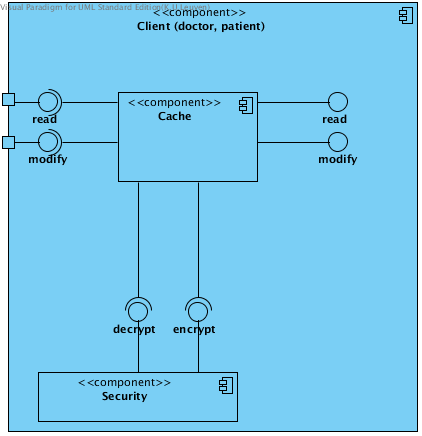
\includegraphics[width=\textwidth]{../images/ClientServer_Client.png}
    \end{figure}
  \end{center}
%TODO opmaken figuur!

\subsection{Element catalog}

\paragraph{Cache}
De cache component is een lokale cache van bestanden die ook op de server aanwezig zijn.

\subsubsection{Element interfaces} 

\paragraph{read}
TODO

\paragraph{modify}
TODO

\paragraph{push}
TODO

\subsubsection{Element behavior}
Wanneer een item uit de cache gelezen wordt (\textit{read}), verstuurt de cache eerst de vraag naar de server als het gegeven item up-to-date is.  Als dit het geval is dan wordt het bestand uit de cache aan de gebruiker weergegeven, is dit niet het geval dan stuurt de server het meest recente bestand terug.  Dit wordt dan opgeslagen in de cache en dan teruggegeven aan de gebruiker.\\
%TODO teruggeven aan de gebruiker??
Het schrijven van een item (\textit{write}) gebeurt door het item eerst lokaal te schrijven, daarna verstuurt de cache een write operatie naar de server.  Wanneer de cache een antwoord gekregen heeft van de server dat de schrijfoperatie correct verlopen is mag de cache het geschreven item uit de cache verwijderen.\\
Een \textit{push} operatie is gelijkaardig aan de schrijf operatie van hierboven.  Het enige verschil is dat het in het geval van een \textit{push} gaat over een operatie waarbij de gebruiker geen toegang heeft tot het te schrijven document.  Hij kan enkel een data-veld toevoegen, een veld wijzigen of overschrijven is niet mogelijk.

\paragraph{Security}
De security component is op zich gelijk aan deze in de server.  De gedetailleerde uitwerking is te vinden in \ref{Client and Server View: Security} Client and Server View: Security.


\subsubsection{Elements and their properties}

\subsubsection{Relations and their properties}

\subsubsection{Element interfaces}

\subsubsection{Element behavior}

\subsection{Context diagram}

\subsection{Variability guide}
Verschillende implementaties van de Client component zijn mogelijk.  Wanneer de client lokaal op een pc wordt uitgewerkt voor een dokter zal de cache waarschijnlijk zo veel mogelijk data bijhouden.\\
Voor een client van de dokter die bijvoorbeeld op een smartphone draait is het onrealistisch om te verwachten dat deze alle data zal cachen.  De client kan dan bijvoorbeeld zo uitgewerkt worden dat de cache van de smartphone iedere morgen voor de huisbezoeken gesynct wordt met de nodige pati\"{e}nten van die dag.\\
Nog een ander geval is het geval van de client voor de apotheek of voor de pati\"{e}nt.  In het geval van een client voor de pati\"{e}nt zal de cache enkel het dossier van de pati\"{e}nt zelf bijhouden.  Voor de apotheek hoeft de cache helemaal geen data te cachen.\\
Een laatste geval is wanneer de cache op een webclient draait.  In dit geval kan de caching aangepast worden naar de mogelijkheden van de webserver.  Hier moet dan wel rekening gehouden worden met de wetgeving die centrale opslag van pati\"{e}nten data verbiedt.  Het is mogelijk dat een webserver zoveel zou gaan cachen dat dit zou kunnen gezien worden als een centrale opslag.  Omdat dit niet toegelaten is moet men er bij de implementatie van deze cache rekening mee houden.  De cache zou zo kunnen aangepast worden om slechts een bepaald aantal documenten bij te houden of enkel de documenten die in een bepaalde tijdspanne opgevraagd zijn.

\subsection{Architecture background}

\subsubsection{Rationale}

\subsubsection{Analysis results}

\subsubsection{Assumptions}

\subsection{Other information}

\subsection{Related view packets}


\section{C\&C Client and Server View: Security}
\label{Client and Server View: Security}

\subsection{Primary presentation}

\begin{center}
    \begin{figure}
      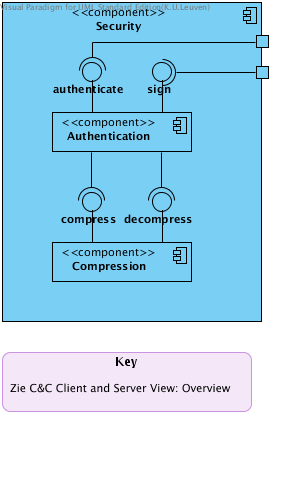
\includegraphics[width=\textwidth]{../images/ClientServer_Security.png}
    \end{figure}
  \end{center}
%TODO opmaken figuur!

\subsection{Element catalog}

\paragraph{Authentication}

\paragraph{Compression}

\subsubsection{Elements and their properties}

\subsubsection{Relations and their properties}

\subsubsection{Element interfaces}

\subsubsection{Element behavior}

\subsection{Context diagram}

\subsection{Variability guide}

\subsection{Architecture background}

\subsubsection{Rationale}

\subsubsection{Analysis results}

\subsubsection{Assumptions}

\subsection{Other information}

\subsection{Related view packets}





\section{VRAAGJES}

Bij deployment data : 
	- is het nodig om nog van de virtuele servers naar security server te gaan?
 	  Authorizatie wordt reeds gechecked in security services, maar moet dit later
	  nog eens herhaald worden???
	- Moeten partiele data servers en figure data server ook nog extra gerepliceerd
	  worden aan de hand van een master-slave configuratie?


\section{Deployment view DMZ}

\subsection{Primary presentation}
\begin{center}
    \begin{figure}
      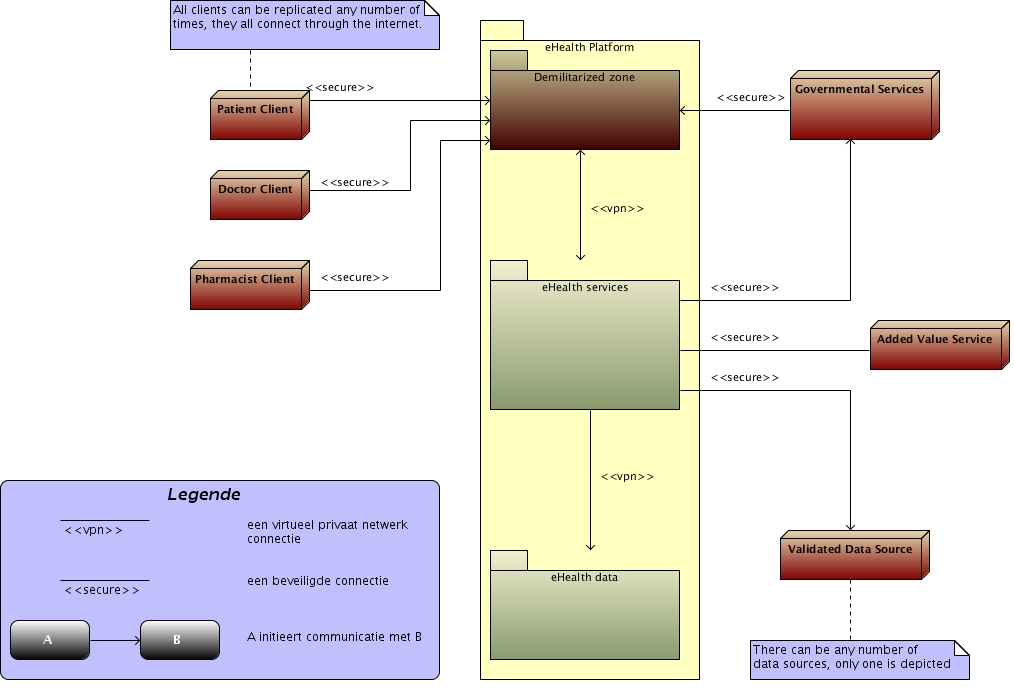
\includegraphics[width=\textwidth]{../images/deployment_DMZ.jpg}
    \end{figure}
  \end{center}

\subsection{Element catalog}

\subsubsection{Elements and their properties}

\begin{enumerate}
\item \textbf{Card Reader}\\
Een gespecialiseerde hardware node die instaat is om data van een elektronische kaart
te lezen en er ook data op te schrijven. Het kan ook data tekenen en encrypteren met
behulp van de keys beschikbaar op de kaart aanwezig in de lezer.
\item \textbf{Patient Client}\\
De PC van een patient.
\item \textbf{Doctor Client}\\
De PC van een dokter.
\item \textbf{Pharmacist Client}\\
De PC van een apotheker.
\item \textbf{Demilitarized Zone}\\
Een gedeelte van het eHealth platform waar publieke services zoals web services en
de API zullen zitten. Deze zone vereist geen authenticatie noch authorizatie, het 
is het toegangspunt tot het platform voor externe gebruikers.
\item \textbf{eHealth Services}\\
Gedeelte van het eHealth platform dat alle business logica (services) bevat.
\item \textbf{eHealth Data}\\
Gedeelte van het eHealth platform dat alle data servers bevat.
\item \textbf{Validated Data Source}\\
Een externe node die gevalideerde medische data aanbiedt. Merk op dat hoewel er slechts 1 node
getekend staat, er zo een heel scala aan data bronnen bestaan.
\item \textbf{Governmental Services}\\
Een externe node waarop de overheid allerhande services aanbiedt zoals het RIZIV en ook een
service waarmee belangrijke data gelogd kan worden.
\end{enumerate}

\subsubsection{Relations and their properties}
Er zijn drie verschillende soorten connecties te onderscheiden : 
\begin{enumerate}
 \item \textbf{Vertrouwde connecties}\\
Dit zijn de connecties op het diagram aangeduid met het stereotype <<trusted>>. Dit zijn
connecties die volledig te vertrouwen zijn. Het gaat hier om de connectie tussen een client
node en de kaart lezer. Hier moeten we qua security niet al te veel aandacht aan geven
aangezien dit gewoon een rechtstreekse connectie is tussen de kaartlezer en de client node,
hier kunnen geen aanvallers aan.
\item \textbf{Beveiligde connecties}\\
Dit zijn de connecties op het diagram aangeduid met het stereotype <<secure>>. Dit zijn
connecties over het internet die goed beveiligd moeten zijn tegen aanvallers. Dit houdt
in dat de twee interagerende nodes moeten weten wie de andere is én dat de communicatie
geëncrypteerd is, zodat luistervinken geen nuttige data te pakken krijgen.
\item \textbf{Virtueel private netwerk connecties}\\
Dit zijn de connectie sop het diagram aangeduid met het stereotype <<vpn>>. Deze connecties
gaan ook over het internet, maar ze maken deel uit van een virtueel privaat netwerk.
\end{enumerate}

\subsubsection{Element interfaces}

Niet van toepassing

\subsubsection{Element behavior}

Niet van toepassing

\subsection{Context diagram}

Nodig bij dit view?

\subsection{Variability guide}

\subsection{Architecture background}

\subsubsection{Rationale}

Het eHealth platform wordt opgedeeld in drie delen. Aan de ene kant hebben we een demilitarized zone (DMZ), aan de andere services en data. Door clients alle clients te laten connecteren langst de demilitarized zone creëren we een centrale plaats vanwaar alle toegang tot het systeem komt. Dit maakt het makkelijker om het systeem te beveiligen. Services en data worden ook van elkaar gescheiden wat resulteert in een grotere modulariteit wat het makkelijker maakt om het geheel te implementeren en te testen.

Om ervoor te zorgen dat de demilitarized zone niet omzeild word door een eventuele aanvaller, wordt er gebruikt gemaakt van virtual private networks (VPNs). Dit bevordert de schaalbaarheid, onderhoudbaarheid en variabiliteit van het systeem aangezien het relatief gemakkelijk is om een nieuwe node toe te voegen moest het nodig zijn. Een VPN wordt ook gebruikt voor alle communicatie tussen de services en data lagen. Een nadeel van de DMZ is dat het een bottleneck vormt voor alle toegang tot het platform. Daarom zullen performantie en beschikbaarheid belangrijke drivers zijn voor de verdere decompositie van de DMZ.

Tenslotte zien we dat de verbinding tussen de eHealth services en de overheid slechts in 1 richting gaat, maar vanuit de overheid kan er wel naar de DMZ gegaan worden. Dit komt doordat de overheid via het internet zal connecteren, waardoor we niet kunnen toelaten dat die alle security maatregelen omzeilt.

\subsubsection{Analysis results}

\subsubsection{Assumptions}

\subsection{Other information}

\subsection{Related view packets}


\section{Deployment view clients}

\subsection{Primary presentation}
\begin{center}
    \begin{figure}
      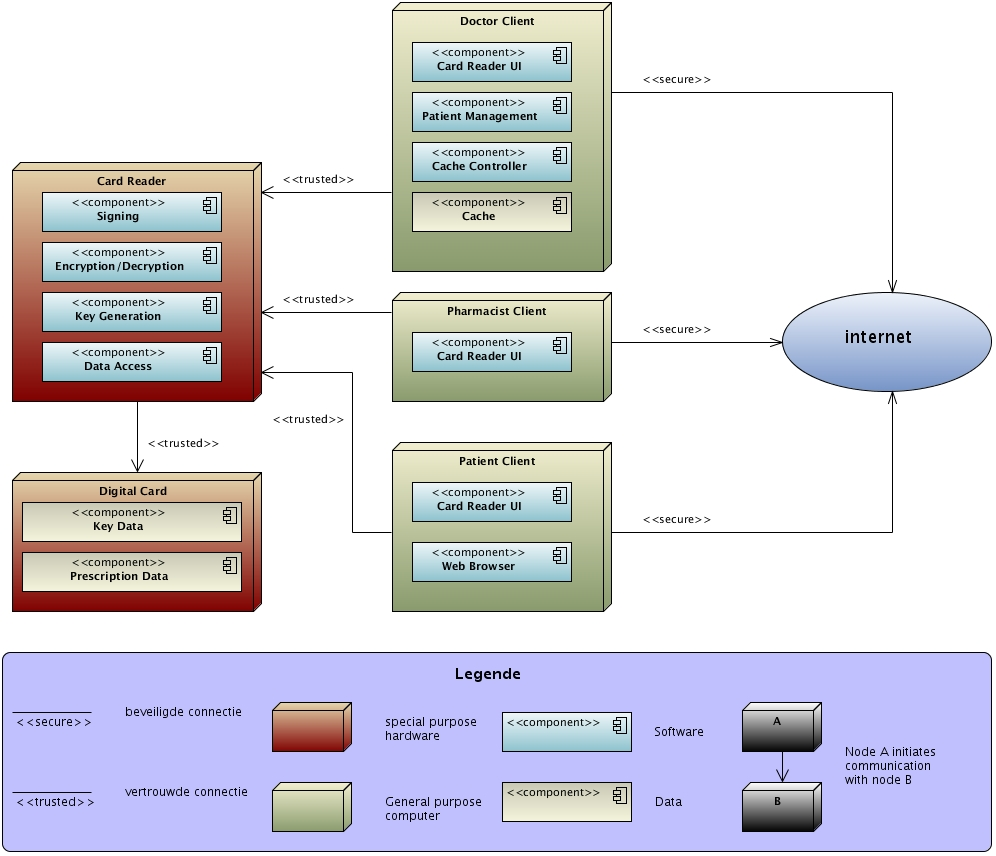
\includegraphics[width=\textwidth]{../images/deployment_clients.jpg}
    \end{figure}
  \end{center}

\subsection{Element catalog}

\subsubsection{Elements and their properties}

\begin{enumerate}
 \item \textbf{Digital Card}\\
Deze node stelt een digitale kaart voor die elke patient en dokter toegewezen krijgt van de overheid. Deze node zal geen echte software bevatten, maar dient enkel als data opslag. Volgende twee soorten data kunnen we onderscheiden :
\begin{enumerate}
 \item \textbf{Key Data}\\
De keys op de kaart. Elke kaart zal een publieke en private sleutel bevatten waarmee getekend en/of geëncrypteerd kan worden met behulp van de elektronische kaartlezer.
\item \textbf{Prescription Data}\\
De voorschriften die een dokter voorschrijft voor een patient zullen op de kaart bijgehouden worden, zodat deze terug uitgelezen kunnen worden bij het ophalen/bestellen van medicatie bij de apotheker/e-pharmacy.
\end{enumerate}

\item \textbf{Card Reader}\\
De elektronische kaartlezer bevat volgende software componenten : 
\begin{enumerate}
\item \textbf{Signing}\\
Software verantwoordelijk voor het tekenen van documenten (voorschriften).
\item \textbf{Encryption/Decryption}\\
Deze component kan data versleutelen en terug ontcijferen met behulp van de keys die op de kaart staan die in de kaartlezer zit.
\item \textbf{Key Generation}\\
Sleutels kunnen ook gegenereerd worden. Dit zal ondermeer gebruikt worden voor het tijdelijk toekennen van toegang tot het globaal medisch dossier.
\item \textbf{Data Access}\\
Deze component is verantwoordelijk voor het ophalen en schrijven van data van/op de elektronische kaart.
\end{enumerate}

\end{enumerate}


\subsubsection{Relations and their properties}

zelfde als bij deployment DMZ, moet dat hier dan herhaald worden?

\subsubsection{Element interfaces}

niet van toepassing

\subsubsection{Element behavior}

niet van toepassing

\subsection{Context diagram}

nodig bij deze view?

\subsection{Variability guide}

\subsection{Architecture background}

\subsubsection{Rationale}



\subsubsection{Analysis results}

\subsubsection{Assumptions}

\subsection{Other information}

\subsection{Related view packets}


\section{Deployment view services}

\subsection{Primary presentation}
\begin{center}
    \begin{figure}
      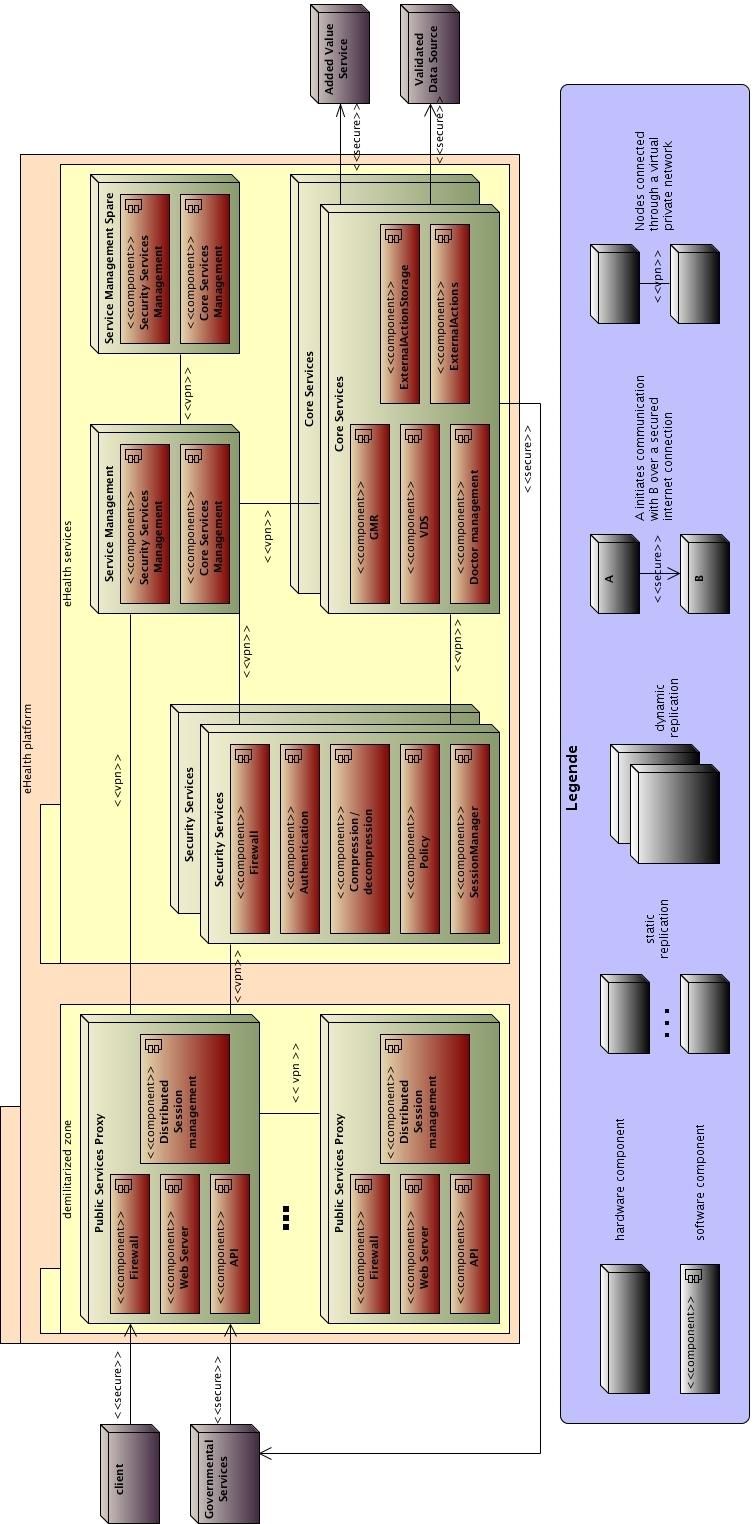
\includegraphics[width=\textwidth]{../images/deployment_services.jpg}
    \end{figure}
  \end{center}

\subsection{Element catalog}

\subsubsection{Elements and their properties}

\subsubsection{Relations and their properties}

\subsubsection{Element interfaces}

\subsubsection{Element behavior}

\subsection{Context diagram}

\subsection{Variability guide}

\subsection{Architecture background}

\subsubsection{Rationale}

\subsubsection{Analysis results}

\subsubsection{Assumptions}

\subsection{Other information}

\subsection{Related view packets}



\section{Deployment view data}

\subsection{Primary presentation}
\begin{center}
    \begin{figure}
      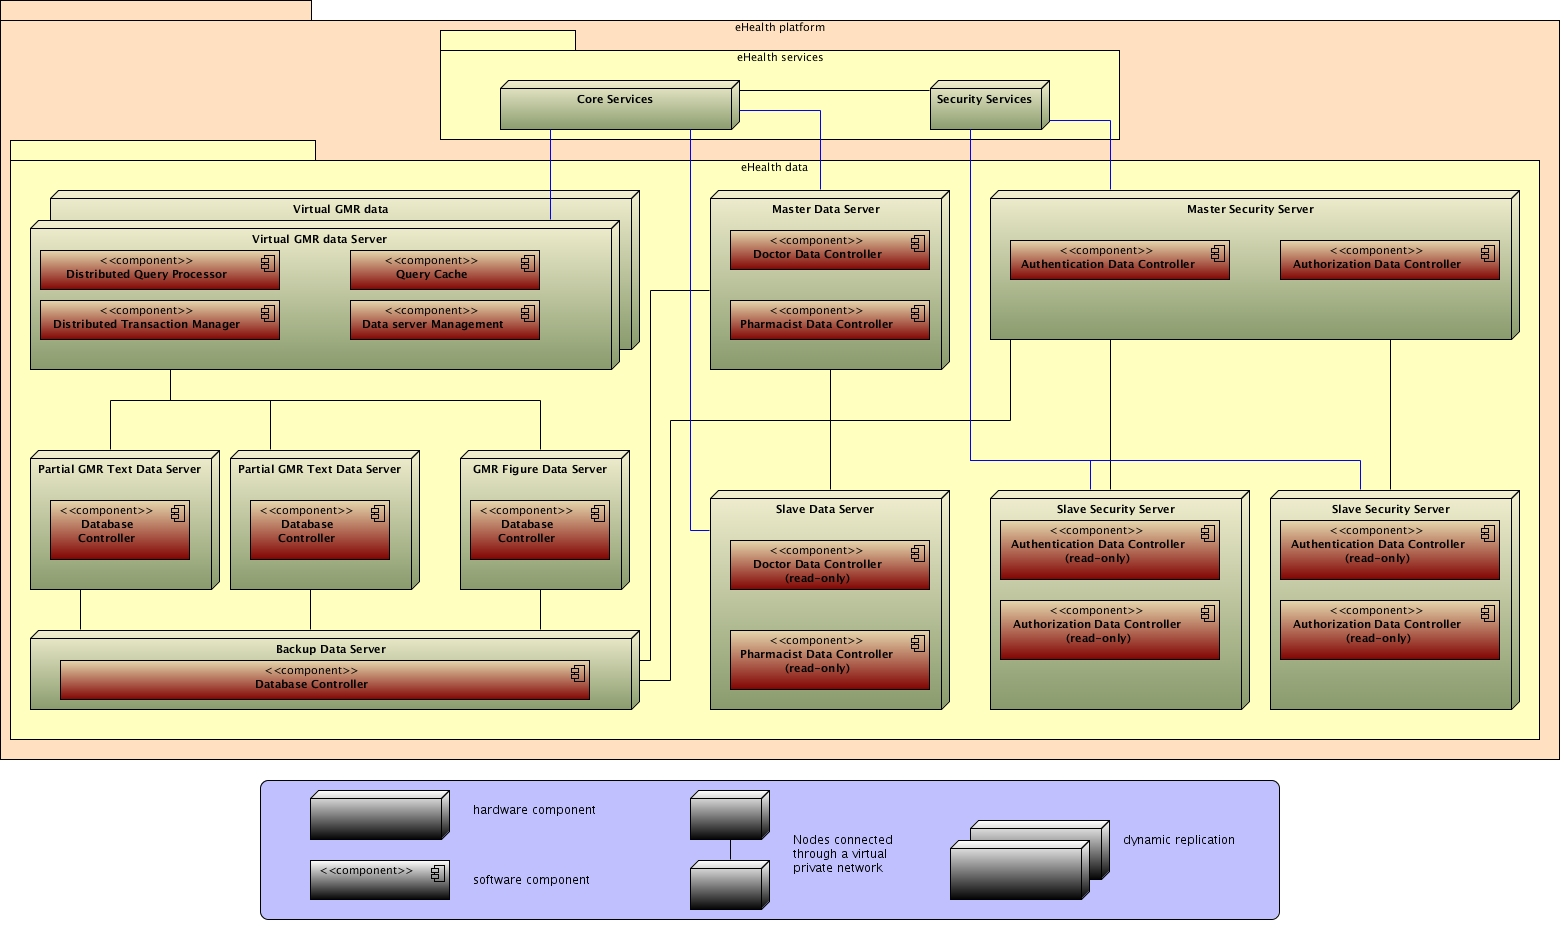
\includegraphics[width=\textwidth]{../images/deployment_data.jpg}
    \end{figure}
  \end{center}

\subsection{Element catalog}

\subsubsection{Elements and their properties}

\subsubsection{Relations and their properties}

\subsubsection{Element interfaces}

\subsubsection{Element behavior}

\subsection{Context diagram}

\subsection{Variability guide}

\subsection{Architecture background}

\subsubsection{Rationale}

\subsubsection{Analysis results}

\subsubsection{Assumptions}

\subsection{Other information}

\subsection{Related view packets}



\section{Interaction Diagrams}

\subsection{Primary presentation}

\subsection{Element catalog}

\subsubsection{Elements and their properties}

\subsubsection{Relations and their properties}

\subsubsection{Element interfaces}

\subsubsection{Element behavior}

\subsection{Context diagram}

\subsection{Variability guide}

\subsection{Architecture background}

\subsubsection{Rationale}

\subsubsection{Analysis results}

\subsubsection{Assumptions}

\subsection{Other information}

\subsection{Related view packets}

\end{document}          
